\documentclass[10pt]{beamer}

\usepackage[no-math]{fontspec}  % no option clash

\usepackage[UTF8]{ctex}



\usepackage{graphicx}
\usepackage{caption}
\usepackage{subcaption}
\usepackage{minted}
\usemintedstyle{manni}
\definecolor{bg}{rgb}{0.95,0.95,0.95}

\usepackage{hyperref}
\hypersetup{pdfpagemode=FullScreen}

\usepackage{float}

\usepackage{amsmath}

\usetheme{metropolis}
\usepackage{appendixnumberbeamer}

\usepackage{booktabs}
\usepackage[scale=2]{ccicons}

\usepackage{pgfplots}
\usepgfplotslibrary{dateplot}

\usepackage{xspace}
\newcommand{\themename}{\textbf{\textsc{metropolis}}\xspace}


\title{ID3}
\subtitle{算法实现及决策树可视化}
\date{\today}
\author{徐遥 SA16214017}
% \institute{None}
\logo{
\includegraphics[height=1.5cm]{./figures/ustc_logo_text.pdf}}

\begin{document}

\maketitle

\begin{frame}{目录}
  \setbeamertemplate{section in toc}[sections numbered]
  \tableofcontents[hideallsubsections]
\end{frame}

\section{使用示例}
\begin{frame}[fragile,allowframebreaks,t]{Golf}
以经典的 Golf 决策树为例,展示所有功能。
\begin{minted}[mathescape,linenos,frame=lines,breaklines,breakautoindent,fontsize=\footnotesize]{Python}
# 利用 pd.read_csv 读取 csv 文件为 DataFrame
train_data = pd.read_csv('golf.csv')
# 初始化 ID3 算法时需要提供训练数据集以及目标属性
id3_solver = ID3(train_data, target='play')
# 进行训练
id3_solver.run()
# 输出训练的到的决策树
id3_solver.render_decision_tree('./dtree')
# 这里为了展示功能,所以直接把训练数据集当作了测试集
result = test_data['play'].values
test_data.drop('play', axis=1, inplace=True)
# 比较预测与实际结果获得正确率
predict = id3_solver.predict(test_data)
accuracy = id3_solver.score(predict, result)            
\end{minted}

\begin{figure}
  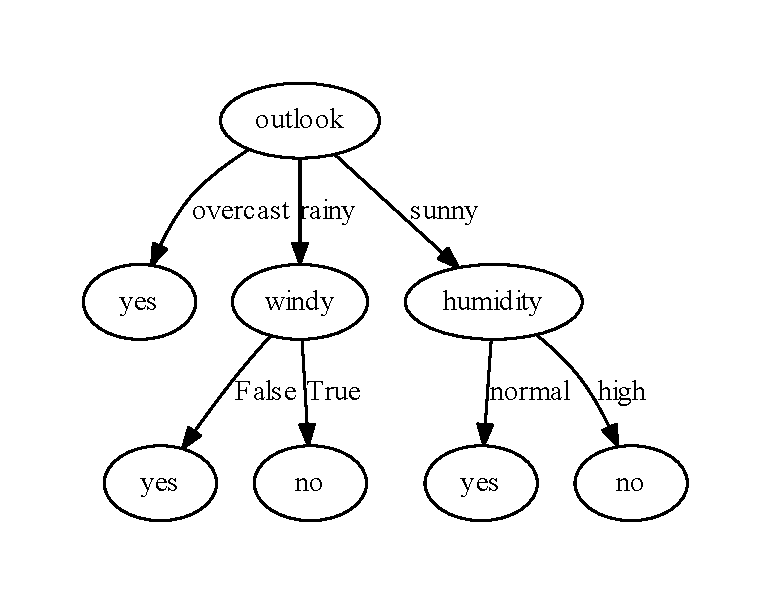
\includegraphics[scale=0.6]{../dtree.pdf}
  \caption{Golf 决策树}
\end{figure}

\end{frame}

\section{数据处理}

\begin{frame}[fragile]{Pandas}
在构造决策树时,需要频繁地计算窗口下计算某属性的熵值。
\begin{align}
  \mathrm{Entropy(A)}&=\sum_{i=1}^{a} \mathrm{Info(data[A])} \\
  \mathrm{Info}&=\sum_{i=1}^{c} - p_i \log_2 p_i
\end{align}
这就要求需要一种能够根据属性值快速筛选数据的数据结构。
因此,我选择了\alert{Pandas (Python Data Analysis Library)} 来处理数据。
\begin{itemize}
  \item 具备按轴或显式数据对齐功能的数据结构;
  \item 数学运算和约简(比如对某个轴求和)可以根据不同元数据(轴编号)进行;
  \item 灵活的处理缺失数据;
  \item 具有多种文件格式的读取能力(CSV、JSON、XLS等等);
\end{itemize}
\end{frame}

\begin{frame}[fragile]{DataFrame}
最终使用的是二维数据结构 DataFrame(属性名即为列名,一个样本即为一行)。
\inputminted[mathescape,linenos,frame=lines,framesep=2mm,breaklines,breakautoindent,fontsize=\small]{Python}{./codes/pandas_demo.py}
\end{frame}

\begin{frame}[fragile,allowframebreaks]{熵的计算}
有了 DataFrame 的帮助计算窗口下各个属性的熵值就变得非常简单。
\begin{minted}[mathescape,linenos,frame=lines,framesep=2mm,breaklines,breakautoindent,fontsize=\small]{Python}
class ID3(object):
    def _entropy(self, data, attribute):
        """计算某个 attribute 的熵,私有
        """
        value_freq = data[attribute].value_counts()
        data_entropy = 0.0
        N = len(data)
        #  $\mathrm{Entropy(A)}=\sum_{i=1}^{s} \mathrm{Info(data[A])}$
        for value, freq in value_freq.items():
            p = freq / N
            data_entropy += p * self._info(data, attribute, value)
        return data_entropy

    def _info(self, data, attribute, attribute_value):
        data = data[data[attribute] == attribute_value]
        target_value_freq = data[self.target].value_counts()
        data_info = 0.0
        N = len(data)
        # $\mathrm{Info}=\sum_{i=1}^{c} - p_i \log_2 p_i$
        for freq in target_value_freq.values:
            p = freq / N
            data_info -= p * math.log(p, 2)
        return data_info                
\end{minted}
\end{frame}

\section{决策树的构造与使用}
\begin{frame}[fragile]{Node}
首先定义了 Node 类,每个节点拥有自己的属性以及子节点。
\begin{minted}[mathescape,linenos,frame=lines,framesep=2mm,breaklines,breakautoindent,fontsize=\small]{Python}
class Node(object):
    def __init__(self, _id):
        self.id = _id
        self.attribute = None
        self.branches = {}           
\end{minted}
其中,branches 为一个 dict, key 为当前节点属性所对应的值。如果节点的 branches 为空,则其 attribute 即为分类。

\end{frame}

\begin{frame}{构造与预测}
  理想的建立决策树的步骤为:
  \begin{enumerate}
    \item 寻找当前窗口下熵值最小的属性,将该属性设为节点,并按其属性值进行数据分割;
    \item 对这些子数据集重复执行上步骤,直到数据集为\alert{同一类别}。
  \end{enumerate}
  理想状态下,使用决策树预测数据的分类就更为简单了,只需要根据数据的属性值一步步从根节点走到叶子节点即可。
\end{frame}




\begin{frame}[fragile]{遇到的问题}
  在数据量较大,属性也较多时,再遵循理想的策略就会遇到问题。
  \metroset{block=fill}
  \begin{columns}[T,onlytextwidth]
    \column{0.48\textwidth}
    \begin{alertblock}{构造}
    有可能遇到所有属性都已被用来划分数据了,但剩下的数据仍然不是同一种类。
    按照理想的步骤,没有办法继续了。
    \end{alertblock}

    \column{0.48\textwidth}
    \begin{alertblock}{预测}
    在沿着决策树预测时,可能会遇到无路可走的情况,即当前节点没有测试数据相对应属性值的子节点。
    \end{alertblock}
  \end{columns}

  \vfill
  为了解决问题,我采用了简单粗暴的策略:
  \alert{那个多选哪个!}
\end{frame}


\begin{frame}[fragile, allowframebreaks]{最终实现}
\begin{minted}[mathescape,linenos,frame=lines,framesep=2mm,breaklines,breakautoindent,fontsize=\footnotesize]{Python}
class ID3(object):
    def _make_decision_tree(self, data, node):
        # 当数据都为同一类数据时,直接返回
        if len(data[self.target].value_counts()) == 1:
            node.attribute = data[self.target].value_counts().index[0]
            return
        # 如果除了 target 外,已经没有其他 attribute 了,那也返回
        if len(data.columns) == 1:
            node.attribute = data[self.target].value_counts().argmax()
            return

        # 寻找熵最小的属性
        min_entropy = math.inf
        for attribute in data.columns:
            if attribute == self.target:
                continue
            temp_entropy = self._entropy(data, attribute)
            if temp_entropy < min_entropy:
                min_entropy = temp_entropy
                node.attribute = attribute
        
        # 建立子节点
        for value in data[node.attribute].value_counts().index:
            branch_data = data[data[node.attribute] == value]
            branch_data = branch_data.drop(node.attribute, axis=1)
            branch_node = self._new_node()
            node.add_branch_node(value, branch_node)
            self._make_decision_tree(branch_data, branch_node)

    def run(self):
        self.root_node = self._new_node()
        self._make_decision_tree(self.data, self.root_node)              
\end{minted}
\end{frame}

\section{决策树的可视化}

\begin{frame}[fragile]{Graphviz}

决策树的可视化利用了贝尔实验室开发的 \href{http://www.graphviz.org/}{Graphviz} 工具包。用户可以使用
DOT 语言来描述图形,然后利用该工具进行图形的布局与绘制,省去手动调整元素的大小与局部的繁琐过程。
对于决策树而言,我们只需要了解如何往有向图(digraph)添加节点与边。
\begin{figure}[!tbp]
  \begin{subfigure}[b]{0.48\textwidth}
    \inputminted[mathescape,breaklines,breakautoindent,fontsize=\tiny]{C}{./figures/graphviz_demo}
    \caption{DOT文件}
  \end{subfigure}
  \hfill
  \begin{subfigure}[b]{0.48\textwidth}
    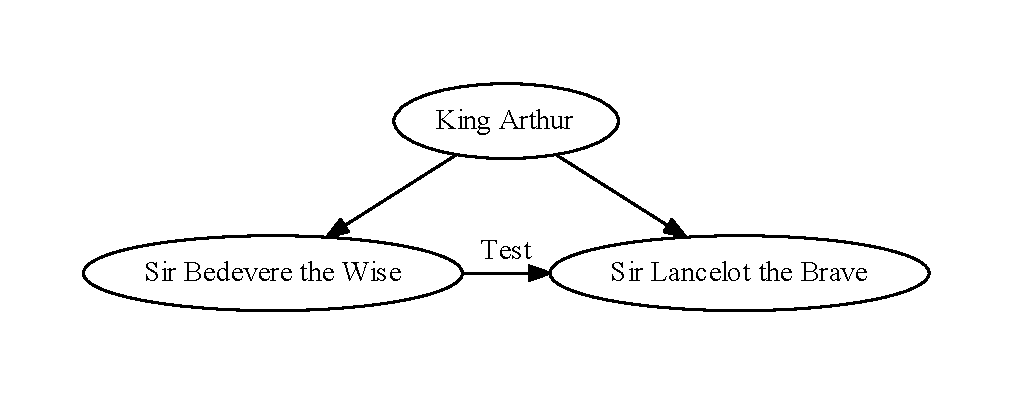
\includegraphics[width=\textwidth]{./figures/graphviz_demo.pdf}
    \caption{渲染后}
  \end{subfigure}
  \caption{Graphviz使用示例}\label{fig:dot_demo}
\end{figure}

\end{frame}

\begin{frame}[fragile]{Graphviz 的 Python 接口}
\mintinline{python}{graphviz} 提供了创建 DOT 文件的 Pyhton 接口。实际上,
图~\ref{fig:dot_demo} 就是其官方示例。
\inputminted[mathescape,linenos,frame=lines,framesep=2mm,breaklines,breakautoindent,fontsize=\small]{python}{./codes/graphviz_demo.py}
\end{frame}


\begin{frame}[fragile,allowframebreaks]{自动生成决策树的 DOT 文件}
有了上述工具,决策树的可视化就变得非常简单了:只需要递归地把所有节点和边加入有向图即可。
\begin{minted}[mathescape,linenos,frame=lines,framesep=2mm,breaklines,breakautoindent,fontsize=\small]{Python}
class ID3(object):
    class Node(object):
        @property
        def node_name(self):
            # 可视化时,每个node,必须要有独一无二的name
            return ''.join([self.attribute, str(self.id)])

        def add_to_graph(self, graph):
            graph.node(self.node_name, self.__str__())
            for edge_name, branch_node in self.branches.items():
                branch_node.add_to_graph(graph)
                graph.edge(self.node_name, branch_node.node_name, label=str(edge_name))

    def render_decision_tree(self, filename):
        if not self.root_node:
            raise ValueError('Tree not decided!')   
        from graphviz import Digraph
        dot_graph = Digraph(comment="Decision Tree")
        self.root_node.add_to_graph(dot_graph)
        dot_graph.render(filename)                    
\end{minted}
\end{frame}

\begin{frame}[allowframebreaks]{生成树展示}
\begin{figure}[H]
  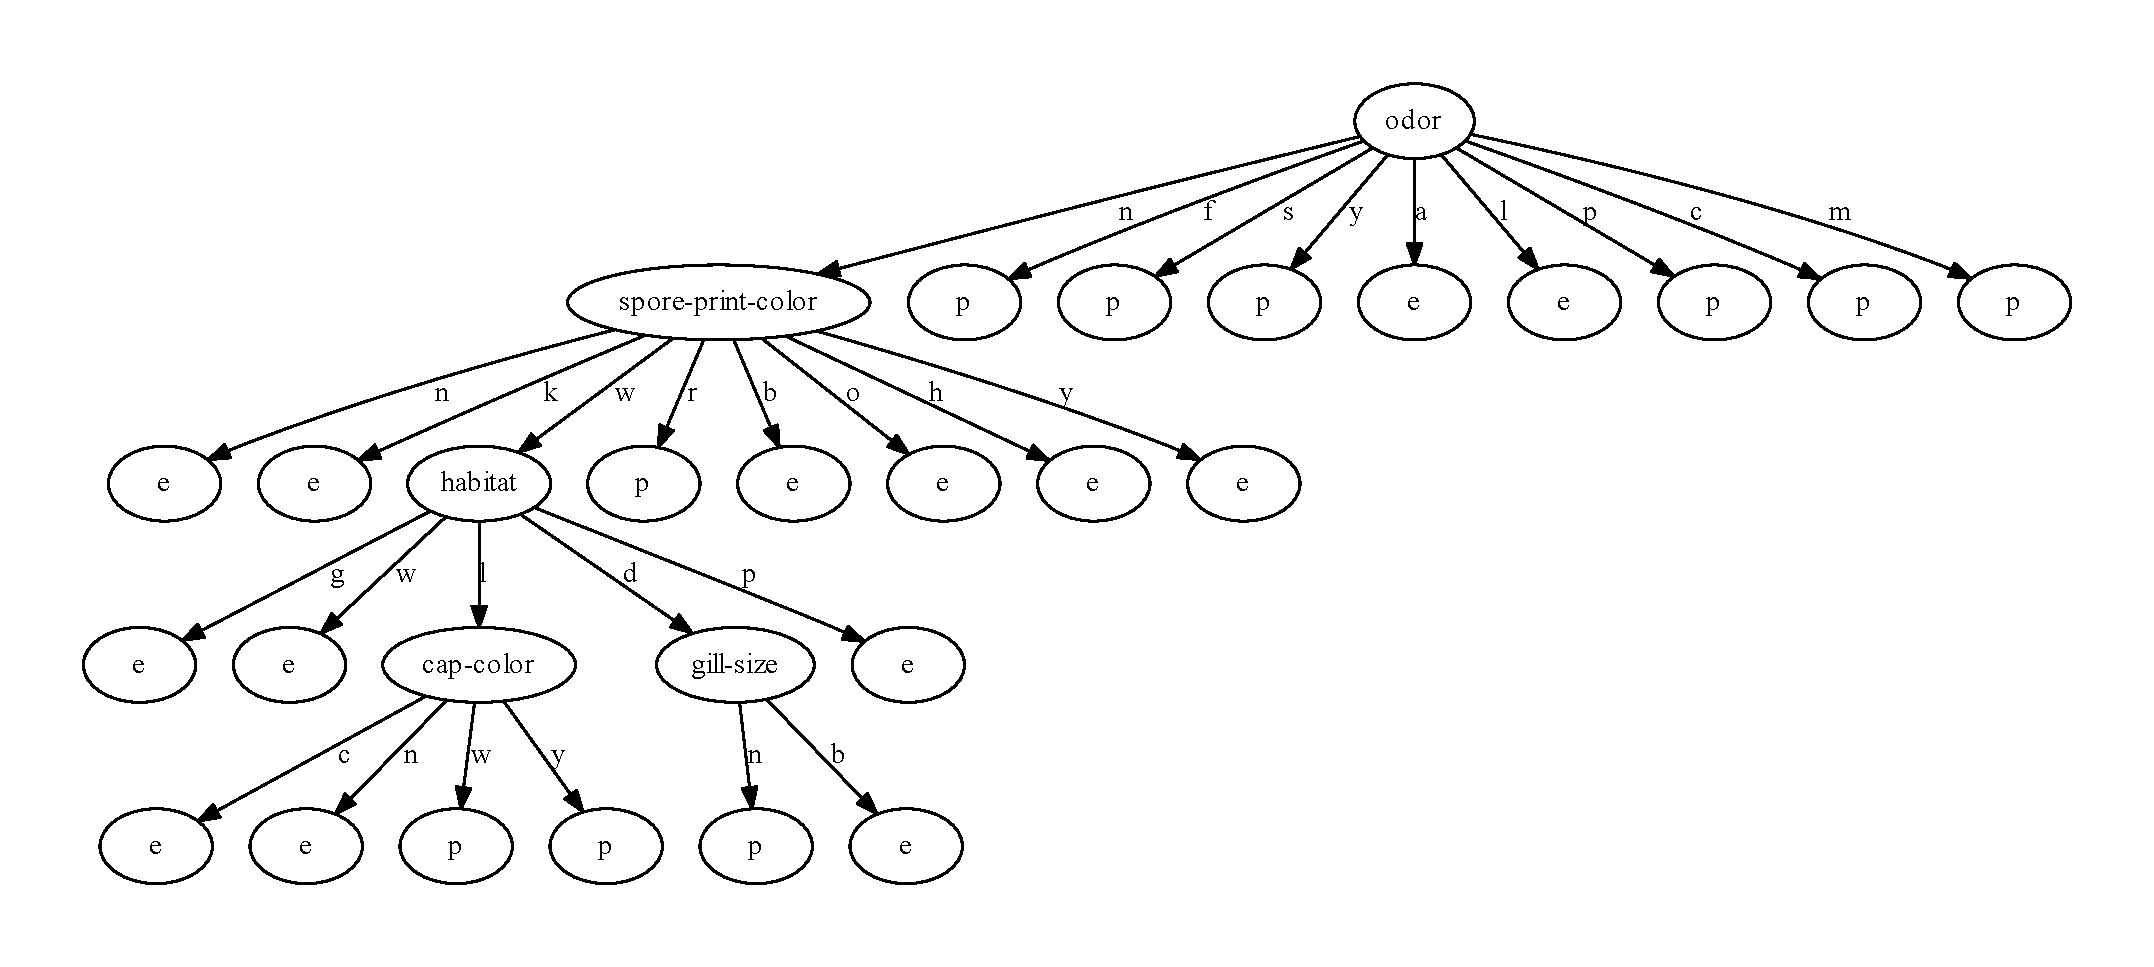
\includegraphics[width=\textwidth]{../mushroom_data/dtree.pdf}
  \caption{蘑菇毒性分类决策树}
\end{figure}       
\end{frame}

\end{document}
